
\chapter{Faculty Workload Model}

\section{Introduction}

In an academic institution, teaching workload only constitutes a small part of the overall workload of a faculty member. In addition to teaching, faculty members are also expected to perform research, manage staff, acquire research funding, and perform various service activities. The workload of a faculty member is therefore a complex function of the various activities that they perform. In an equal distribution of workload, each faculty member would be expected to perform the same amount of work in each of the activities. However, this would be a disservice to the institution as it would not take into account the differences in the abilities of the faculty members, as well as their preferences for the various activities. In addition, the workload of a faculty member is not static, but changes over time as they progress in their career. For example, a junior faculty member would be expected to spend more time on teaching than research, while a senior faculty member would be expected to make significant research and service contributions. Thus, a fair and equitable workload distribution should take the research and service contributions of the faculty members into account.

In the pursuit of an equitable workload distribution, the first step is to quantify the workload of the various activities. This is a non-trivial task as the various activities are not easily quantifiable. The Faculty Workload Model aims to solve this problem by providing a framework for quantifying the workload of the various activities.

\section{Objectives of the Faculty Workload Model}

The aim of the Faculty Workload Model is to provide transparency and accountability in the workload allocation process, and to ensure equity and fairness in the distribution of workload and resources.



\section{Principles Guiding the Faculty Workload Model}
\label{sec:principles_guiding_workload_allocation_model}

To achieve the objectives of the workload allocation model, it is important to define a set of principles and attributes that the workload allocation model should satisfy. These principles and attributes are:

\begin{enumerate}

      \item The workload allocation model should be accurate.

            The workload allocation model should be able to accurately quantify the workload of the various activities. This is important as the workload allocation model will influence the distribution of teaching workload to the faculty, and the allocation of resources to the various departments. An inaccurate workload allocation model will result in an unfair distribution of workload and resources.

      \item The workload allocation model should be transparent and easily understood.

            Complexity is the enemy of transparency. A complex workload allocation model might be able to accurately quantify the workload of the various activities, but it will be difficult for the faculty to understand how the workload is being allocated. This causes the faculty to lose confidence in the workload allocation model, and will result in a lack of buy-in from the faculty. Additionally, a complex workload allocation model will be difficult to fine-tune and adapt to the needs of the institution.

      \item The workload allocation model should be flexible and adaptable to the needs of the institution.

            Carrying on from the previous point, the workload allocation model should be flexible and adaptable to the needs of the institution. Different institutions have different priorities and needs, and the workload allocation model should be able to adapt to these needs. For example, a teaching-focused institution might want to place more emphasis on teaching workload, while a research-focused institution might want to place more emphasis on research workload. The workload allocation model should be able to adapt to these different needs.

      \item The workload allocation model should account for the zero-sum nature of workload.

            The working hours of a faculty member are finite. As such, the workload of the various activities are zero-sum in nature. For example, a faculty member who spends more time on teaching will have less time to spend on research. The workload allocation model should account for this zero-sum nature of workload. This is important as the workload allocation model will influence the distribution of teaching workload to the faculty, and the allocation of resources to the various departments. An inaccurate workload allocation model will result in an unfair distribution of workload and resources.

      \item The workload allocation model should be inclusive and account for the contributions of all faculty members.

            An academic institution is made up of faculty members of different roles and seniority. The faculty are also broadly classified into lecturers and professors and the institution's goals and priorities for the faculty are influenced by the faculty's role and seniority. For example, a lecturer would be expected to spend more time on teaching than research, while a professor would be expected to make significant research and service contributions. The workload allocation model should be able to account for the contributions of all faculty members, regardless of their roles and seniority.

\end{enumerate}


\section{Distinguishing Workload Patterns among Faculty Types}

An academic institution consists of faculty members of different roles and seniority. The faculty are broadly classified into lecturers and professors, and the institution's goals and priorities for the faculty are influenced by the faculty's role and seniority. For example, a lecturer would be expected to spend more time on teaching than research, while a professor would be expected to make significant research and service contributions. The workload allocation model should be able to

% TODO

\section{Modelling Research Workload}
\label{sec:modelling_research_workload}

The research workload of a faculty is a complex function of the various research activities that they perform. In order to quantify the research workload of a faculty, we first need to identify the various research activities that they perform. The research activities of a faculty can be broadly classified into the following categories:

\begin{enumerate}

      \item Research Supervision

            This includes the supervision of post doctoral fellows, research fellows and research assistants. The workload of research supervision is dependent on the number of research staff that the faculty is supervising, as well as the seniority of the research staff. For example, a faculty member who is supervising a post doctoral fellow would be expected to spend less time on research supervision than a faculty member who is supervising a research assistant, as the post doctoral fellow would be expected to be more independent than the research assistant.

      \item Research Funding

            This includes the acquisition of research funding from external sources. This further involves the writing of research proposals, as well as the application and management of research grants. The management of research grants includes hiring the research staff for the projects associated with the research grants, as well as bookkeeping and reporting of the research grants. One way to quantify the research funding workload of a faculty is to use the amount of research funding that they have acquired. However, this is not an accurate measure of the research funding workload as the amount of research funding that a faculty has acquired is dependent on the research funding opportunities that are available to them. For example, a faculty member who is in a research area that is currently popular would be expected to acquire more research funding than a faculty member who is in a research area that is currently not popular.

            Another approach is to use the number of research grants that a faculty has acquired or applied to, as a measure of the research funding workload. However, this is also not an accurate measure of the research funding workload as different research grants have different levels of complexity and scrutiny in their application process. This is especially true for research grants that are awarded through a competitive process, as the application process for these research grants are more complex and require more effort than research grants that are awarded through a non-competitive process. All things being equal, a faculty member who has applied for more research grants would be expected to have a higher research funding workload than a faculty member who has applied for less research grants. However, this activity remains difficult to quantify due to the variations in the research funding sources.

      \item Research Publication

            This includes the writing of research papers, as well as the submission of research papers to conferences and journals. The workload of research publication is dependent on the number of research papers that the faculty has published, as well as the quality and subject matter of the research papers. For example, a faculty member who has published a research paper in a top-tier conference would generally be expected to have a higher research publication workload than a faculty member who has published a research paper in a lower-tier conference. However, this activity remains difficult to quantify due to the variations in the research publication venues as well as the subject matter of the research papers.

\end{enumerate}

Additionally, another component of research workload is the research service workload. This includes the service activities that the faculty performs for the research community. For example, the faculty might be serving on the program committee of a conference, or the editorial board of a journal, or might be reviewing research papers for conferences and journals. The workload of research service is dependent on the number of research service activities that the faculty is performing, as well as the seniority of the research service activities. However, this activity is classified as service workload and is not considered as part of the research workload.

\subsection{Methods of Quantifying Research Workload}

The research workload of a faculty is a complex function of the various research activities that they perform. The research workload of a faculty can be quantified using the following methods:

\subsection{Comprehensive Research Workload}

One approach to quantifying the research workload of a faculty is to comprehensively quantify the workload of the various research activities. This approach is the most accurate approach to quantifying the research workload of a faculty, as it takes into account the various research activities that the faculty performs. For the activities defined in \autoref{sec:modelling_research_workload}, the research workload of a faculty can be defined as:

\begin{enumerate}

      \item Research Supervision Workload (\(R_{sup}\))

            Research supervision workload is dependent on the number of research staff that the faculty is supervising, as well as the seniority of the research staff. We found that the research supervision for a post-doctoral fellow is approximately 0.5 times the research supervision for a research assistant. As such, the research supervision workload of a faculty can be quantified using the following formula:

            \begin{equation*}
                  R_sup = 0.5 \times N_{PD} +  N_{RA}
            \end{equation*}

            where $N_{PD}$ is the number of post-doctoral fellows that the faculty is supervising, and $N_{RA}$ is the number of research assistants that the faculty is supervising.


      \item Research Funding Workload (\(R_{fund}\))

            Research funding workload is dependent on the number of research grants that the faculty has applied to, as well as the complexity of the research grants. Since the complexity of the research grants is difficult to quantify, we will only use the number of research grants that the faculty has applied to as a measure of the research funding workload. The research funding workload of a faculty can be quantified using the following formula:

            \begin{equation*}
                  R_{fund} = N_{rg}
            \end{equation*}

            where $N_{rg}$ is the number of research grants that the faculty has applied to.

      \item Research Publication Workload (\(R_{pub}\))

            Research publication workload is dependent on the number of research papers and journal articles that the faculty has published, as well as the quality and subject matter of the publications. Since the effort required to publish a research paper or journal article depends on the quality and subject matter of the publication, we can assign a peer-rated weight to each publication based on the quality and subject matter of the publication. The research publication workload of a faculty can be quantified using the following formula:

            \begin{equation*}
                  R_{pub} = \sum_{i=1}^{N_{rp}} w_i
            \end{equation*}

            where $N_{rp}$ is the number of research papers and journal articles that the faculty has published, and $w_i$ is the peer-rated weight of the $i$-th publication.

            As a simplification of the above formula, we can ignore the peer-rated weight of the publications and use the number of publications as a measure of the research publication workload. The research publication workload of a faculty in this case would simply be

            \begin{equation*}
                  R_{pub} = N_{rp}
            \end{equation*}

\end{enumerate}

However, each of these research activities are not directly comparable as the nature of each of these activities are different. Therefore, to quantify the research workload of a faculty, we need to convert the research workload of each of these activities into a common unit. For this, we can take a simple take a simple weighted average of the research workload of each of these activities, where the weights correspond to the relative workload per unit of each of these activities. However, defining the workload at this level of granularity has considerable disadvantages. These disadvantages are discussed in \autoref{sec:research_workload_derived_from_research_supervision}.


\subsection{Research Workload Derived from Research Supervision}
\label{sec:research_workload_derived_from_research_supervision}

Although the research workload of a faculty can be comprehensively quantified using the methods described in the previous section, this leads to a complex workload allocation model that is fairly complex. However, a complex model is difficult for the faculty to understand, and will result in a lack of transparency and buy-in from the faculty. Additionally, a complex model will be difficult to fine-tune and adapt to the needs of the institution, as tuning the weights of the various research activities will be difficult.

Moreover, including the workload of research publication is problematic as it is a trailing indicator of research workload. This is because the research publications are only published after the research has been completed. This trailing nature of research publication workload means that if the faculty is given teaching workload relaxation to account for their significant research outputs, the workload relaxation will only be given for the following semester or term, which can cause misplaced distribution of the workload. For example, if the major conferences in the faculty member's research area are held in the first half of the year, the faculty member will be given teaching workload relaxation in the second half of the year, where their research workload is typically lower. Moreover, looking at the lower research outputs in the second half of the year, the faculty member might be given additional teaching workload in the first half of the following year, where their research workload is already high. This problem could be circumvented by accounting for the research workload of the previous year, but that leads to it's own set of issues. This misplaced distribution of workload can be avoided by using a leading indicator of research workload, such as research supervision workload.

Another observation is that the research publication and research funding workload of a faculty has a direct correlation with the research supervision workload of the faculty. This is because the research supervision workload will directly impact the number of research publications that the faculty will be able to author or co-author. Additionally, the research supervision workload is also proportional to the research funding workload, as the number of research staff that can be hired is dependent on the research funding that the faculty has acquired. As a result, a clear way to simplify the research workload allocation model is to use the research supervision workload as a proxy for the research workload of the faculty. Thus, the research workload of a faculty can be quantified using the following formula:

\begin{equation*}
      R = 0.5 \times N_{PD} +  N_{RA}
\end{equation*}

where $N_{PD}$ is the number of post-doctoral fellows that the faculty is supervising, and $N_{RA}$ is the number of research assistants that the faculty is supervising.

This has the advantage of being a simple workload allocation model that is easy to understand and fine-tune, as the only parameter that needs to be tuned is the workload of supervising a post-doctoral fellow relative to the workload of supervising a research assistant. Additionally, this is also a leading indicator of the total research workload of the faculty.

\subsection{Addressing Hierarchy Effects in Research}

As described above, quantifying the research workload of a faculty as a function of the research staff working under them has considerable advantages. We used a simple linear function to quantify the research workload of a faculty. However, one key observation from how faculty supervise a large cohort of research staff was that the faculty do not directly supervise all of the research staff. Instead, the faculty supervise a small number of senior research staff, who in turn supervise a larger number of junior research staff. This not only reduces the workload of the faculty, but also provides a career progression path for the research staff and an opportunity for the senior research staff to gain supervisory experience. To account for this hierarchy effect, a non-linear function can be used to quantify the research workload of a faculty. The non-linear function is expected to have the following properties:

\begin{enumerate}

      \item The research workload of a faculty should be a monotonically increasing function of the number of research staff that they are supervising
      \item The research workload of a faculty should rise linearly for a small number of research staff, and then rise non-linearly for a large number of research staff to account for the hierarchy effect
      \item The research workload of a faculty should asymptotically approach a maximum value as beyond a certain number of research staff, the research workload of the faculty will not increase significantly

\end{enumerate}

The non-linear function that satisfies the above properties is the logistic function, which is defined as:

\begin{equation*}
      f(x) = \frac{L}{1 + e^{-k(x-x_0)}}
\end{equation*}

where $L$ is the maximum value of the function, $k$ is the steepness of the curve, and $x_0$ is the midpoint of the curve where the function increases linearly. The logistic function is plotted in \autoref{fig:logistic_function}.

\begin{figure}[htpb]
      \centering
      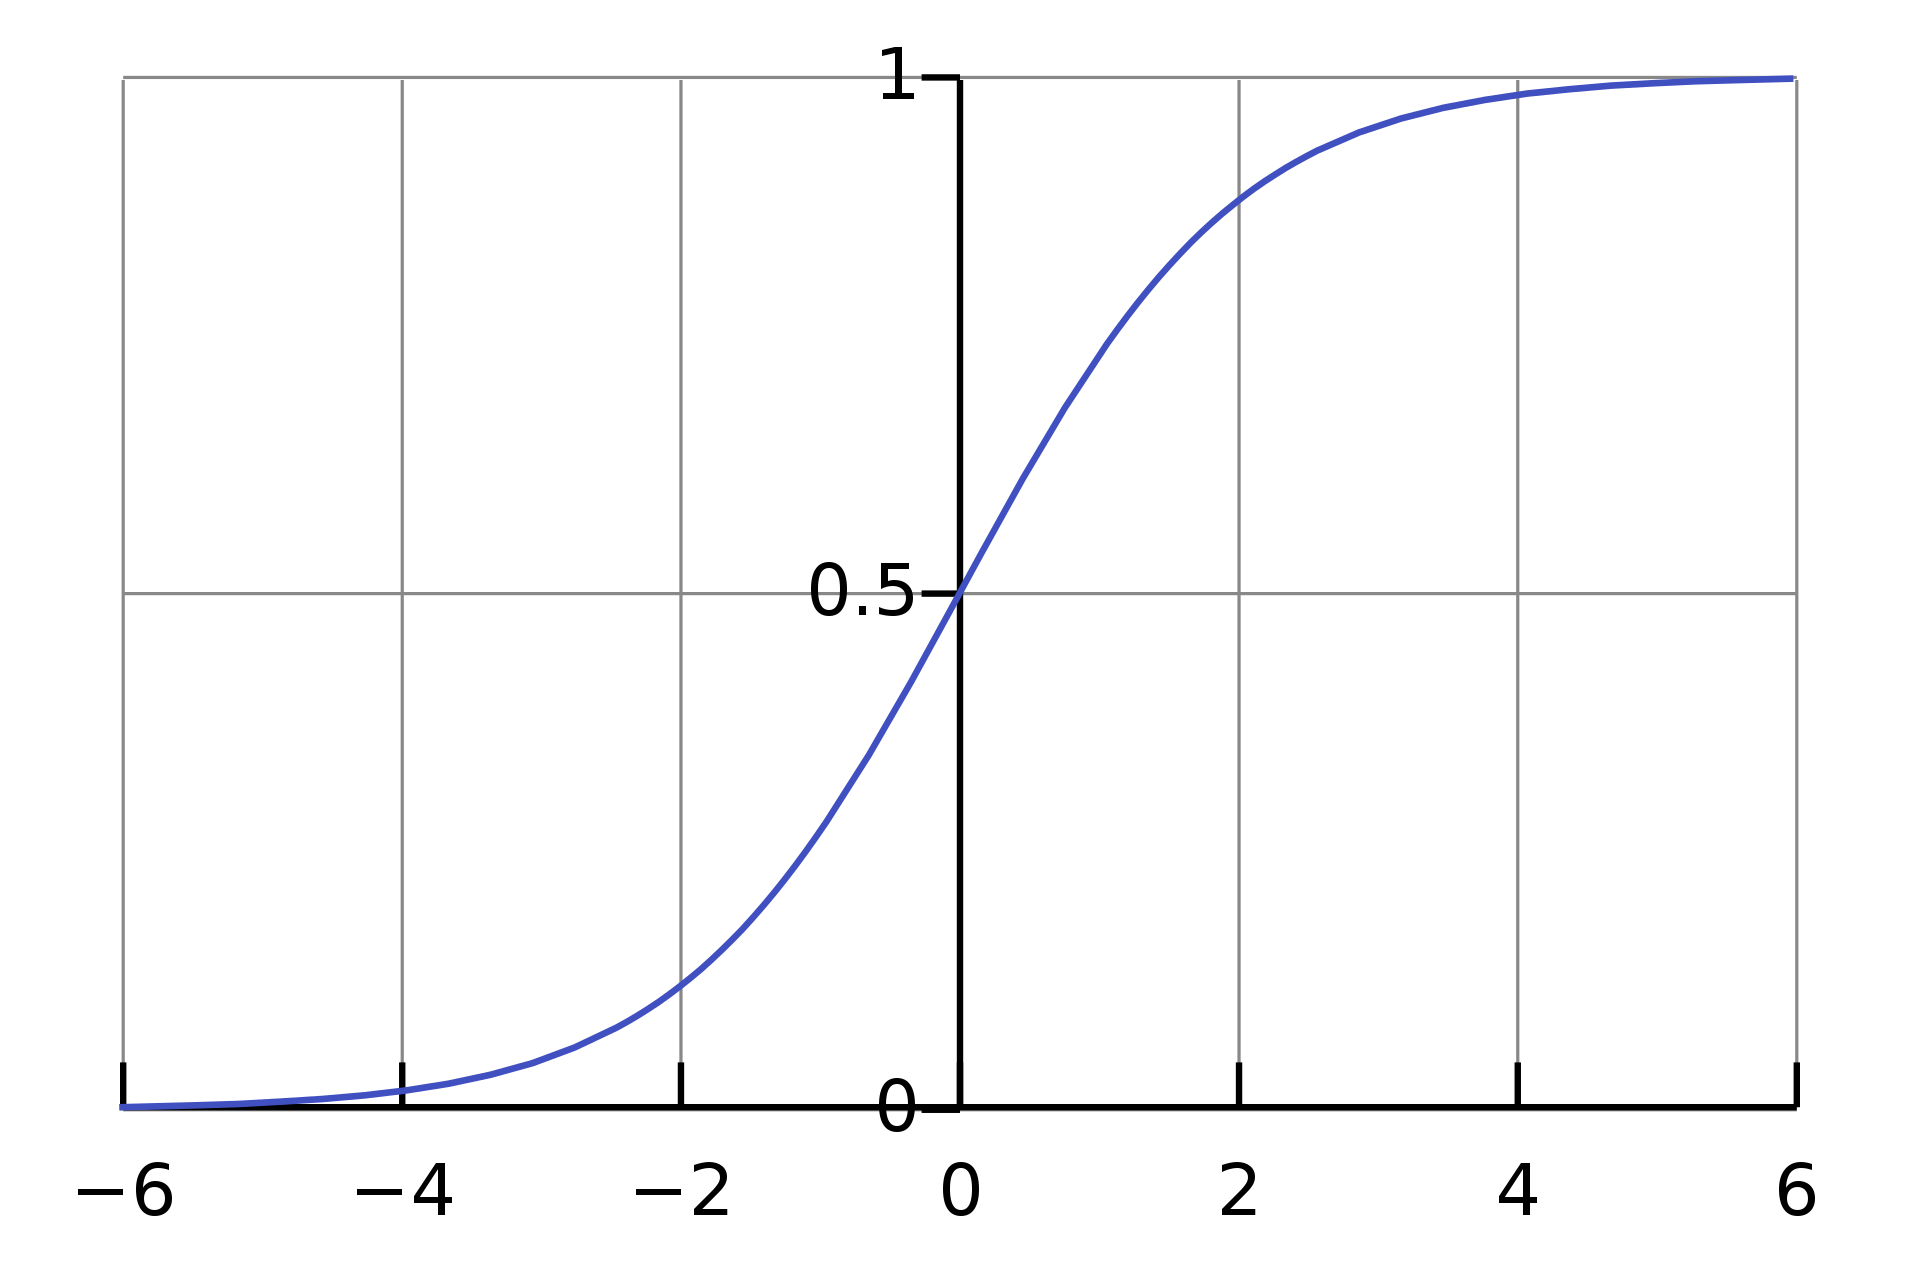
\includegraphics[width=0.5\linewidth]{images/tanh_plot.png}
      \caption{Logistic Function for L = 1, k = 1, x0 = 0}
      \label{fig:logistic_function}
\end{figure}

For the research workload of a faculty, we apply the logistic function to the number of research staff that the faculty is supervising. We also normalize the function so that the maximum value of the function is 1, and the function has a midpoint of 0 since the research workload of a faculty should be 0 when they are not supervising any research staff. We also tweak the steepness of the curve so that the research workload so that the research workload approaches the maxima at around 10 research staff. The research workload of a faculty can be quantified using the following formula:

\begin{equation}
      R = \frac{2}{1 + e^{-x/3}} - 1
\end{equation}

where $ x = 0.5 \times N_{PD} +  N_{RA}$, $N_{PD}$ and $N_{RA}$ are the number of post-doctoral fellows and research assistants respectively that the faculty is supervising.

\begin{figure}[htpb]
      \centering
      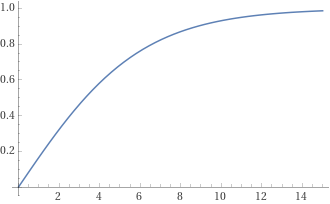
\includegraphics[width=0.5\linewidth]{images/research_workload_plot.png}
      \caption{Research Workload ($R$)}
      \label{fig:research_workload_plot}
\end{figure}


\section{Modelling Service Workload}

The service workload of a faculty consists of the various service activities that they perform. The service activities of a faculty include but are not limited to the following:

\begin{enumerate}

      \item Departmental Service

            This is the various service activities that the faculty performs for the department. It includes serving on departmental committees, as well as performing administrative duties for the department.

      \item Administrative Duties

            This is the various administrative duties that the faculty performs for the institution. It includes duties like serving on various committees and panels the admissions panel, the scholarship review panel and the examinations committee, coordinating a research center etc.

      \item Research Service Duties

            This is the various service activities that the faculty performs for the research community. It includes serving on the program committee of a conference, or the editorial board of a journal, or reviewing research papers for conferences and journals.

\end{enumerate}

The service workload of a faculty is dependent on the number of service duties that the faculty is performing, as well as the amount of effort required to perform each of these duties. Since the nature of each service duty is different, it is difficult to quantify the service workload of a faculty through a heuristic approach. Instead, we can use a simple weighted average of the service workload of each of these duties, where the weights correspond to the workload per semester for each of these duties. The service workload of a faculty can be quantified using the following formula:

\begin{equation*}
      \text{Service Workload} = \sum_{i=1}^{N_{sd}} w_i
\end{equation*}

where $N_{sd}$ is the number of service duties that the faculty is performing, and $w_i$ is the workload per semester of the $i$-th service duty.

Some of the service duties are performed by all faculty members. For example, all faculty members are expected to perform some research service duties, be it reviewing research papers or serving on the program committee of a conference. These service duties are excluded from the workload allocation model as they are not indicative of the workload of an individual faculty member. The allocation of service duties also depends on the seniority of the faculty member. For example, a junior faculty member would be expected to generally perform less service duties and contribute primarily towards teaching and research, while as the faculty member progresses in their career, they would be expected to perform more service duties like serving on departmental committees and major administrative duties like coordinating a research center, or even serving as the Chair of the department. A typical faculty member would be expected to perform 0-2 service duties per semester, while senior faculty members would be expected to perform 2-4 service duties per semester.

Some of the service duties and their corresponding workload per semester are shown in \autoref{tab:service_duties}.

\begin{table}[htpb]
      \centering
      \begin{tabular}{|l | l | r |}
            \hline
            Designation     & Service Duty                                  & Workload \\
            \hline
            Member          & Industrial Attachment Steering Committee      & 1.00     \\
            Member          & Research Mentorship and Consultancy Committee & 1.00     \\
            Member          & Nanyang Research Programme Committee          & 1.00     \\
            Coordinator     & Final Year Projects                           & 1.00     \\
            Director        & Research Centre                               & 1.00     \\
            Group Lead      & Research Focus Group                          & 1.25     \\
            Member          & Research Integrity Committee                  & 1.00     \\
            Member          & Scholarship Interview Panel                   & 1.00     \\
            Member          & School Review Committee                       & 1.00     \\
            Member          & School Reappointment Committee                & 1.00     \\
            Member          & School Search Committee                       & 1.00     \\
            Chairperson     & Student Outreach Committee                    & 1.25     \\
            Coordinator     & Time-Tabling                                  & 1.00     \\
            Associate Chair & Associate Chair                               & 1.00     \\
            \hline
      \end{tabular}
      \caption{Service Duties and Workload}
      \label{tab:service_duties}
\end{table}

\section{RTS Model for Faculty Workload}

With the research and service workload of a faculty quantified, we can model the overall workload of a faculty. In the absence of overtime, it is fair to assume that the total workload of a faculty should be closely comparable since it is the same number of working hours. Thus, the faculty workload model serves greater value in showing the comparative distribution of the workload of various faculty, and the corresponding distribution of their workload across teaching, research and service. Therefore, instead of trying to quantify the workload of the faculty in terms of the number of hours, we choose to quantify the ratio of the workload of the faculty across the various activities. This is because the workload of the faculty is a zero-sum game, and additional workload of the faculty in one activity will result in a reduction of workload in the other activities.

Thus, we define the workload of a faculty as a ratio of the workload of the faculty across Research ($R$), Service ($S$) and Teaching ($T$), where the total workload of the faculty sums up to 12 units i.e.

\begin{equation*}
      \begin{aligned}
            \text{Faculty Workload} & = R:T:S \\
            R + T + S               & = 12
      \end{aligned}
\end{equation*}

% TODO

% 1. Define

\section{Teaching Workload derived from RTS Model}



\section{Health Metrics Derived from the Workload Model}
